% !TeX root = tesis.tex

En numerosos contextos algebraicos, ciertas operaciones resultan computacionalmente sencillas, mientras que sus inversas pueden ser significativamente más complejas. Un ejemplo es el problema del logaritmo discreto (\DLP). Intuitivamente, elevar un elemento de un grupo a una potencia es una operación eficiente. Sin embargo, determinar qué exponente fue utilizado (aun conociendo el resultado) puede ser computacionalmente difícil. Esta asimetría constituye la base de múltiples construcciones criptográficas.

El problema del logaritmo discreto ha sido ampliamente estudiado en la literatura criptográfica \cite{hac,katz}.

\begin{definition}[\DLP]
\label{def:apendice-a-dlp-dlp}
	Sea $(\GG, \cdot)$ un grupo cíclico finito, y sea $g$ un generador de $\GG$. Dado $h \in \GG$, el problema del logaritmo discreto consiste en hallar un $x \in \Z$ que satisfaga $h = g^x$. Al valor $x$ se lo denomina logaritmo discreto de $h$ en base $g$, denotado $\log_g(h)$ cuando existe y es único módulo $\ord{\GG}$.
\end{definition}

A diferencia del logaritmo en los números reales, donde existen algoritmos eficientes para su cálculo, en grupos finitos no se conocen métodos generales eficientes para resolver el \DLP. La dificultad del problema depende fuertemente de la estructura del grupo subyacente.

En grupos cíclicos genéricos, \DLP se considera computacionalmente difícil en el sentido de la complejidad algorítmica. Se sabe que cualquier algoritmo probabilístico que resuelva \DLP con alta probabilidad requiere, en el peor caso, un número de operaciones del orden de $\BigOmega(\sqrt{n})$, donde $n$ es el orden del grupo cíclico \cite{shoup1997lowerbounds}. No se sabe si el \DLP pertenece a la clase de complejidad $\Pclass$, ni si es $\NP$-completo.

Un algoritmo clásico que muestra que esta barrera es alcanzable en el modelo genérico de grupo es el algoritmo \textit{Baby-Step Giant-Step} (\BSGS). Sea $\GG = \gen{g}$ un grupo cíclico de orden $n$, y sea $h \in \GG$. Queremos hallar $x \in \Z$ tal que $h = g^x$. Si $m = \left\lceil \sqrt{n} \right\rceil$, entonces todo $0 \leq x < n$ puede escribirse como $x = im + j$ para algunos $0 \leq i,j < m$. Por lo tanto:
$$h = g^x = g^{im + j} = (g^m)^i g^j,$$
y el \DLP equivale a buscar índices $i,j$ tales que $h(g^{-m})^i = g^j$.

\begin{figure}[!t]
	\centering
	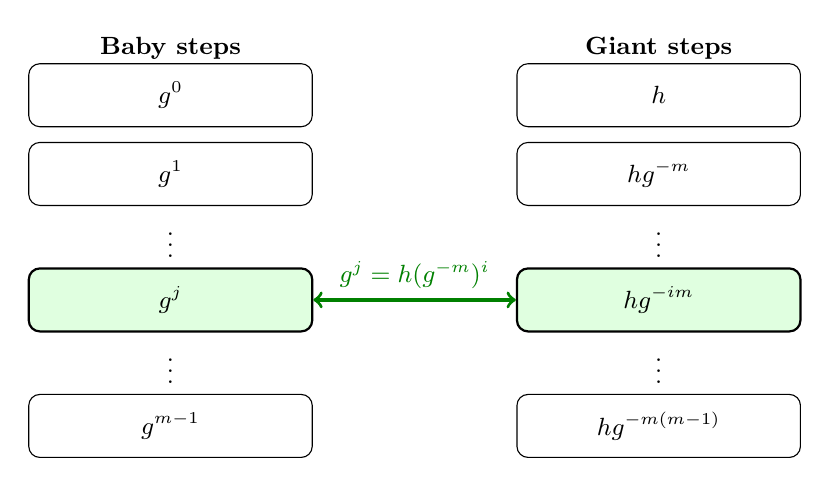
\begin{tikzpicture}[
		scale=1,
		transform shape,
		every node/.style={font=\small, align=center},
		box/.style={draw, rounded corners=4pt, minimum width=3.6cm, minimum height=0.8cm},
		match/.style={draw, rounded corners=4pt, thick, fill=green!12, minimum width=3.6cm, minimum height=0.8cm},
		lbl/.style={font=\footnotesize\itshape}
	]
		\node at (-3.1, 1.6) {\textbf{Baby steps}};
		\node at (3.1, 1.6) {\textbf{Giant steps}};

		\node[box] (b0) at (-3.1, 1) {$g^0$};
		\node[box] (b1) at (-3.1, 0) {$g^1$};
		\node at (-3.1, -0.8) {$\vdots$};
		\node[match] (bj) at (-3.1, -1.6) {$g^j$};
		\node at (-3.1, -2.4) {$\vdots$};
		\node [box] at (-3.1, -3.2) {$g^{m-1}$};

		\node[box] (g0) at (3.1, 1) {$h$};
		\node[box] (g1) at (3.1, 0) {$hg^{-m}$};
		\node at (3.1, -0.8) {$\vdots$};
		\node[match] (gi) at (3.1, -1.6) {$hg^{-im}$};
		\node at (3.1, -2.4) {$\vdots$};
		\node [box] at (3.1, -3.2) {$hg^{-m(m-1)}$};
		
		\draw[<->, very thick, green!50!black] (bj) -- node[above] {$g^j = h(g^{-m})^i$} (gi);
	\end{tikzpicture}
	\caption{Idea del algoritmo \textit{Baby-Step Giant-Step} para resolver un \DLP en un grupo cíclico $\GG=\gen{g}$. La tabla de la izquierda enumera los \textit{baby steps} $g^j$, la de la derecha enumera los \textit{giant steps} $h(g^{-m})^i$, y una coincidencia determina un exponente $x=im+j$ tal que $h=g^x$.}
	\label{fig:bsgs-intuition}
\end{figure}

\begin{algorithm}[h]
	\caption{Algoritmo Baby-Step Giant-Step para \DLP}
	\label{alg:bsgs-dlp}
	\begin{algorithmic}[1]
		\Require Grupo cíclico finito $\GG = \gen{g}$ de orden $n$, elemento $h \in \GG$
		\Ensure Un exponente $x \in \Z$ tal que $h = g^x$, si existe
		\State $(m, \gamma, y) \gets \left(\left\lceil \sqrt{n} \right\rceil, g^{-m}, h\right)$
		\State $T \gets \{(g^j, j): 0 \leq j < m\}$
		\For{$i = 0$ \textbf{to} $m-1$}
			\If{$y \in T$}
				\State Sea $j$ tal que $T[y] = j$
				\State \Return $x = im + j$
			\EndIf
			\State $y \gets y \cdot \gamma$
		\EndFor
		\State \Return $\bot$
	\end{algorithmic}
\end{algorithm}

Cuando el grupo considerado es el grupo multiplicativo de un cuerpo finito, por ejemplo $\Fmul{q}$, la estructura aritmética adicional permite algoritmos más eficientes que en un grupo genérico. En el caso particular de cuerpos primos grandes, el mejor algoritmo clásico conocido es el Number Field Sieve para logaritmos discretos (\NFSDL), cuya complejidad es subexponencial.

El \DLP ocupa un lugar central en la criptografía moderna, ya que la seguridad de numerosos esquemas depende de su dificultad computacional. Entre ellos se encuentran el intercambio de claves de Diffie-Hellman, diversos esquemas de clave pública y varios esquemas de firma digital, como Schnorr y DSA. En este marco, una clave privada suele modelarse como un exponente $x \in \N$, mientras que la clave pública asociada es el elemento $g^x$.

En síntesis, calcular potencias en un grupo cíclico es eficiente, mientras que invertir esa operación resulta computacionalmente prohibitivo con recursos realistas. Esta asimetría entre cómputo directo e inversión es precisamente lo que vuelve útil al \DLP como fuente de seguridad criptográfica.
